\chapter{A Survey on Stress Testing Software Systems}

Load, performance, and stress testing are typically done to locate bottlenecks in a system, to support a performance-tuning effort, and to collect other performance-related indicators to help stakeholders get informed about the quality of the application being tested \cite{Sandler2004} \cite{Corporation2007}. 


The performance testing aims at verifying a specified system performance. This kind of test is executed by simulating hundreds of simultaneous users or more over a defined time interval \cite{DiLucca2006}. The purpose of this assessment is to demonstrate that the system reaches its performance objectives \cite{Sandler2004}.  Term often used interchangeably with “stress” and “load” testing. Ideally “performance” testing is defined in requirements documentation or QA or Test Plans \cite{Lewis2005}.


In a load testing, the system is evaluated at predefined load levels \cite{DiLucca2006}. The aim of this test is to determine whether the system can reach its performance targets for availability, concurrency, throughput, and response time. Load testing is the closest to real application use \cite{Molyneaux2009}. A typical load test can last from several hours to a few days, during which system behavior data like execution logs and various metrics are collected \cite{Afzal2009a}. 

Stress testing investigates the behavior of the system under conditions
that overload its resources. The stress testing verifies the system behavior against heavy workloads \cite{Sandler2004} \cite{Lewis2005}, which are executed to evaluate a system beyond its limits, validate system response in activity peaks, and verify whether the system is able to recover from these conditions. It differs from other kinds of testing in that the system is executed on or beyond its breakpoints, forcing the application or the supporting infrastructure to fail \cite{DiLucca2006} \cite{Molyneaux2009}.


This chapter surveys the state of the art literature in stress testing research. The thesis extends the survey presented by Jiang et al. to the Stress Testing context \cite{Jiang2010}.  This survey will be useful for stress testing practitioners and software engineering researchers with interests in testing and analyzing software systems. We proposed the following four research questions:


\begin{itemize}
\item How is a proper stress designed?
\item How is a stress test executed and automated?
\item What are the main problems found by stress tests?
\item How are the stress tests results analysed?
\end{itemize}

The population in this study is the domain of software testing. Intervention includes application of stress test techniques to test different types of non-functional properties.


\section{Background}


Stress testing is boundary testing. Some of the resources that stress testing subjects to heavy loads include \cite{Lewis2005}:

\begin{itemize}
\item Memory
\item Networks
\item Transaction queues
\item Transaction schedulers
\item User of the system
\end{itemize}

The following are the suggested steps for stress testing \cite{Lewis2005}:

\begin{itemize}
\item Perform simple multitask tests.
\item After the simple stress defects are corrected, stress the system to
the breaking point.
\item Perform the stress tests repeatedly for every development spiral.
\end{itemize}

While load testing is the process of assessing non-functional quality related problems under load. Performance testing is used to measure and/or evaluate performance
related aspects (e.g., response time, throughput and resource utilizations) of algorithms, designs/architectures, modules, configurations, or the overall systems. Stress tests puts a system under extreme conditions to verify the robustness of the system and/or detect various functional bugs (e.g., memory leaks and deadlocks) \cite{Afzal2009a}. The next subsections present details about the stress test process, automated stress test tools and the stress test results.

\subsection{Stress Test Process}

Contrary to functional testing, which has clear testing objectives, Stress testing objectives are not clear in the early development stages and are often defined later on a case-by-case basis. The Fig. \ref{fig:testprocess} shows a common Load, Performance and Stress test process  \cite{Jiang2010}.

\begin{figure}[!ht]
\centering
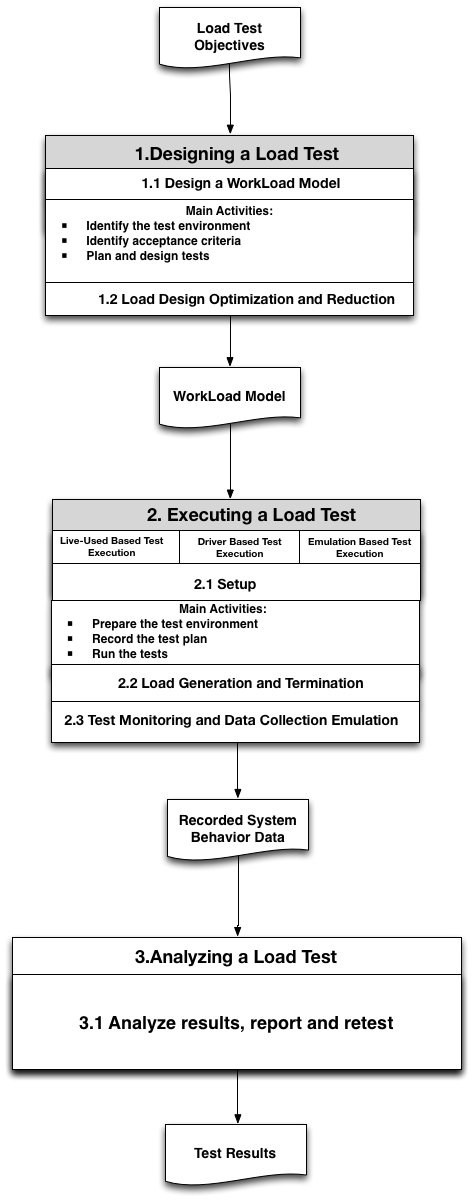
\includegraphics[width=0.5\textwidth]{./images/testprocess.png}
\caption{Load, Performance and Stress Test Process \cite{Jiang2010}\cite{Erinle2013}}
\label{fig:testprocess}
\end{figure}


The goal of the load design phase is to devise a load, which can uncover non-functional problems. Once the load is defined, the system under test executes the load and the system behavior under load is recorded. Load testing practitioners then analyze the system behavior to detect problems \cite{Jiang2010}. 

Once a proper load is designed, a load test is executed. The load test execution phase consists of the following three main aspects: (1) Setup, which includes system deployment and test execution setup; (2) Load Generation and Termination, which consists of generating the load; and (3) Test Monitoring and Data Collection, which includes recording the system behavior during execution\cite{Jiang2010}. 

The core activities in conducting an usual Load, Performance and Stress tests are \cite{Erinle2013}: 

\begin{itemize}
\item Identify the test environment: identify test and production environments and knowing the hardware, software, and network configurations helps derive an effective test plan and identify testing challenges from the outset.

\item Identify acceptance criteria: identify the response time, throughput, and resource utilization goals and constraints.

\item Plan and design tests:identify the test scenarios.In the context of testing, a scenario is a sequence of steps in an application. It can represent a use case or a business function such as searching a product catalog, adding an item to a shopping cart, or placing an order \cite{Corporation2007}. This task includes a description
of the speed, availability, data volume throughput rate, response
time, and recovery time of various functions, stress, and so on. This
serves as a basis for understanding the level of performance and
stress testing that may be required to each test scenario \cite{Lewis2005}.

\item Prepare the test environment: configure the test environment, tools, and resources necessary to conduct the planned test scenarios.

\item Record the test plan: record the planned test scenarios using a testing tool.

\item Run the tests: Once recorded, execute the test plans under light load and verify the correctness of the test scripts and output results.

\item Analyze results, report, and retest: examine the results of each successive run and identify areas of bottleneck that need addressing.  

\end{itemize}





\section{Research Question 1:How is a proper stress designed?}

The design of a stress test depends intrinsically on the load model applied to the software under test. Based on the objectives, there are two general schools of thought for designing a proper load to achieve such objectives \cite{Afzal2009a}:

\begin{itemize}
\item Designing Realistic Loads (Workload Descriptive). 
\item Designing Fault-Inducing Loads ( Workload Generative).
\end{itemize}

In Designing Realistic Loads, the main goal of testing is to ensure that the system can function correctly once. Designing Fault-Inducing Loads  aims to design loads, which are likely to cause functional or non-functional problems \cite{Afzal2009a}.

Stress testing projects should start with the development of a model for user workload that an application receives. This should take into consideration various performance aspects of the application and the infrastructure that a given workload will impact. A workload is a key component of such a model \cite{Molyneaux2009}.

The term workload represents the size of the demand that will be imposed on the application under test in an execution. The metric  used for measure a workload is dependent on the application domain, such as the length of the video in a transcoding application for multimedia files or the size of the input files in a file compression application \cite{Feitelson2013} \cite{Molyneaux2009} \cite{Goncalves2014}. 

Workload is also defined by the load distribution between the identified transactions at a given time. Workload helps researchers study the system behavior identified in several load models. A workload model can be designed to verify the predictability, repeatability, and scalability of a system \cite{Feitelson2013} \cite{Molyneaux2009}.


Workload modeling is the attempt to create a simple and generic model that can then be used to generate synthetic workloads. The goal is typically to be able to create workloads that can be used in performance evaluation studies. Sometimes, the synthetic workload is supposed to be similar to those that occur in practice in real systems \cite{Feitelson2013} \cite{Molyneaux2009}.

There are two kinds of workload models: descriptive and generative. The main difference between the two is that descriptive models just try to mimic the phenomena observed in the workload, whereas generative models try to emulate the process that generated the workload in the first place \cite{DiLucca2006}. 

In descriptive models, one finds different levels of abstraction on the one hand and different levels of fidelity to the original data on the other hand. The most strictly faithful models try to mimic the data directly using the statistical distribution of the data. The most common strategy used in descriptive modeling is to create a statistical model of an observed workload (Fig. \ref{fig:descriptivemodel}). This model is applied to all the workload attributes, e.g., computation, memory usage, I/O behavior, communication, etc. \cite{DiLucca2006}. Fig. \ref{fig:descriptivemodel} shows a simplified workflow of a descriptive model. The workflow has six phases. In the first phase, the user uses the system in the production environment. In the second phase, the tester collects the user's data, such as logs, clicks, and preferences, from the system. The third phase consists in developing a model designed to emulate the user's behavior. The fourth phase is made up of the execution of the test, emulation of the user's behavior, and log gathering.



\begin{figure}[!ht]

\centering
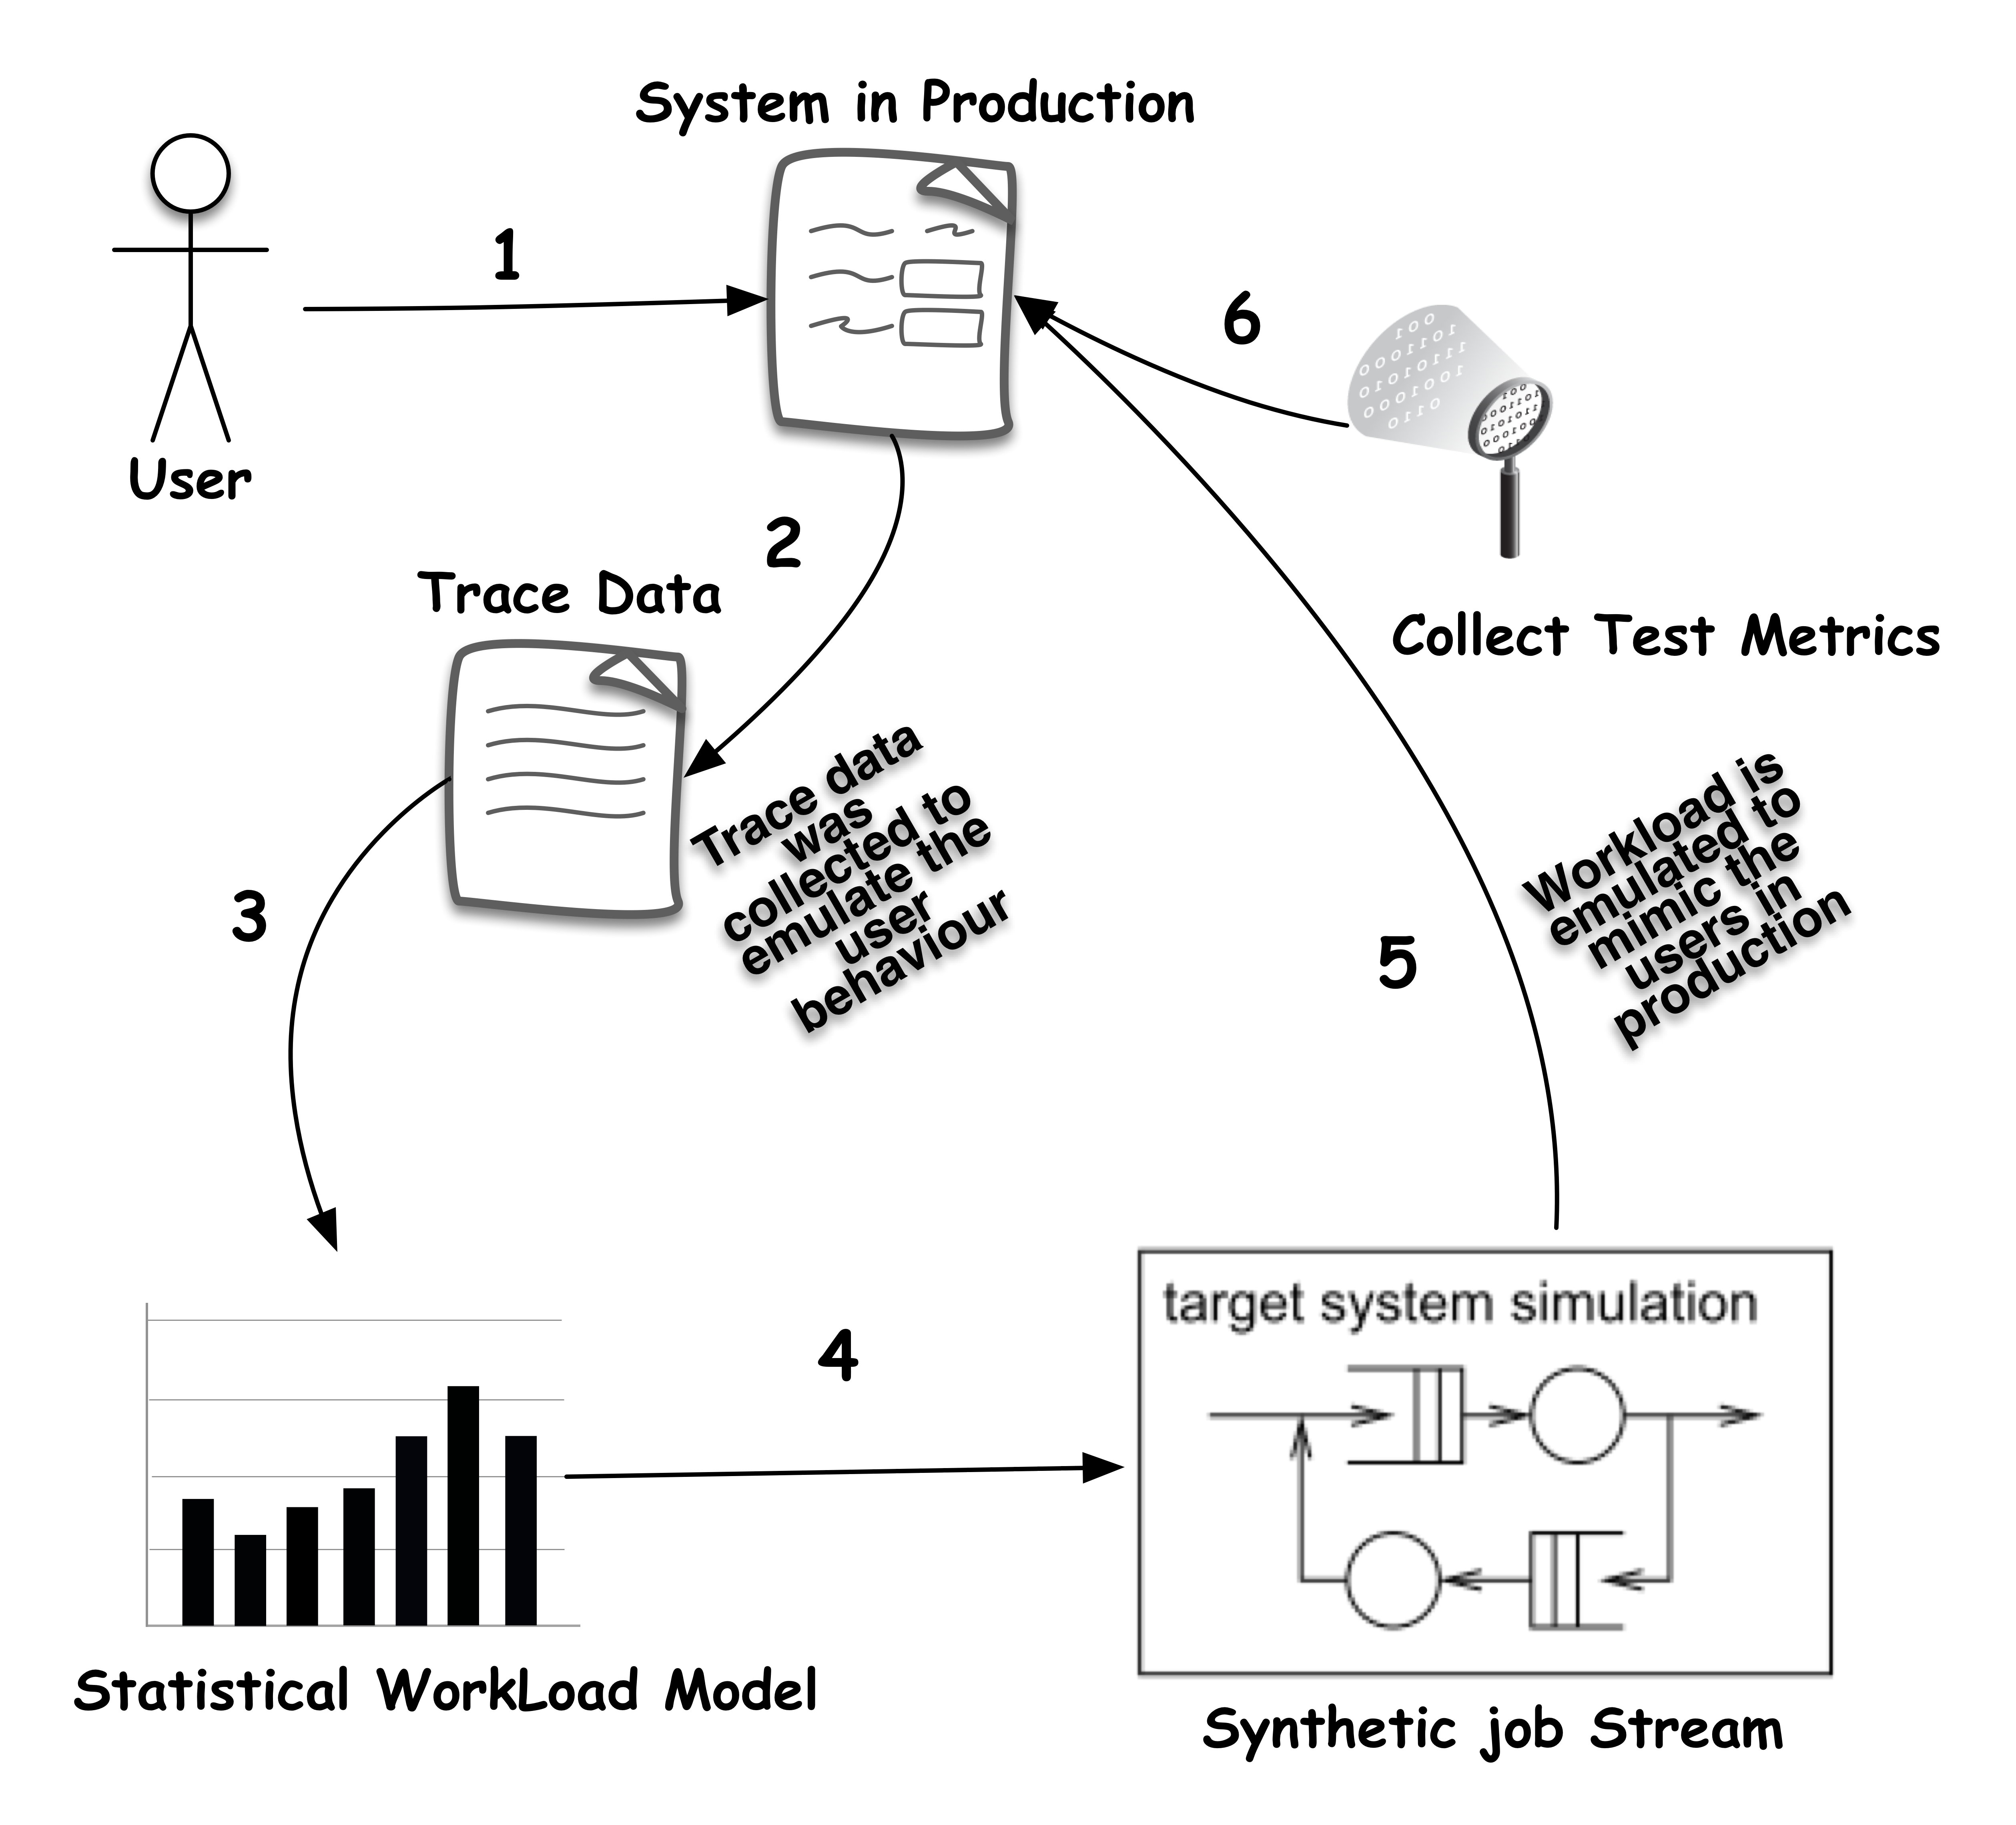
\includegraphics[width=0.8\textwidth]{./images/workloadmodel1300dpi.png}
\caption{Workload modeling based on statistical data \cite{DiLucca2006}}
\label{fig:descriptivemodel}
\end{figure}


Generative models are indirect in the sense that they do not model the statistical distributions. Instead, they describe how users will behave when they generate the workload. An important benefit of the generative approach is that it facilitates manipulations of the workload. It is often desirable to be able to change the workload conditions as part of the evaluation. Descriptive models do not offer any option regarding how to do so. With the generative models, however, we can modify the workload-generation process to fit the desired conditions \cite{DiLucca2006}. The difference between the workflows of the descriptive and the generative models is that user behavior is not collected from logs, but simulated from a model that can receive feedback from the test execution (Fig. \ref{fig:generativemodel}).


\begin{figure}[!ht]
\centering
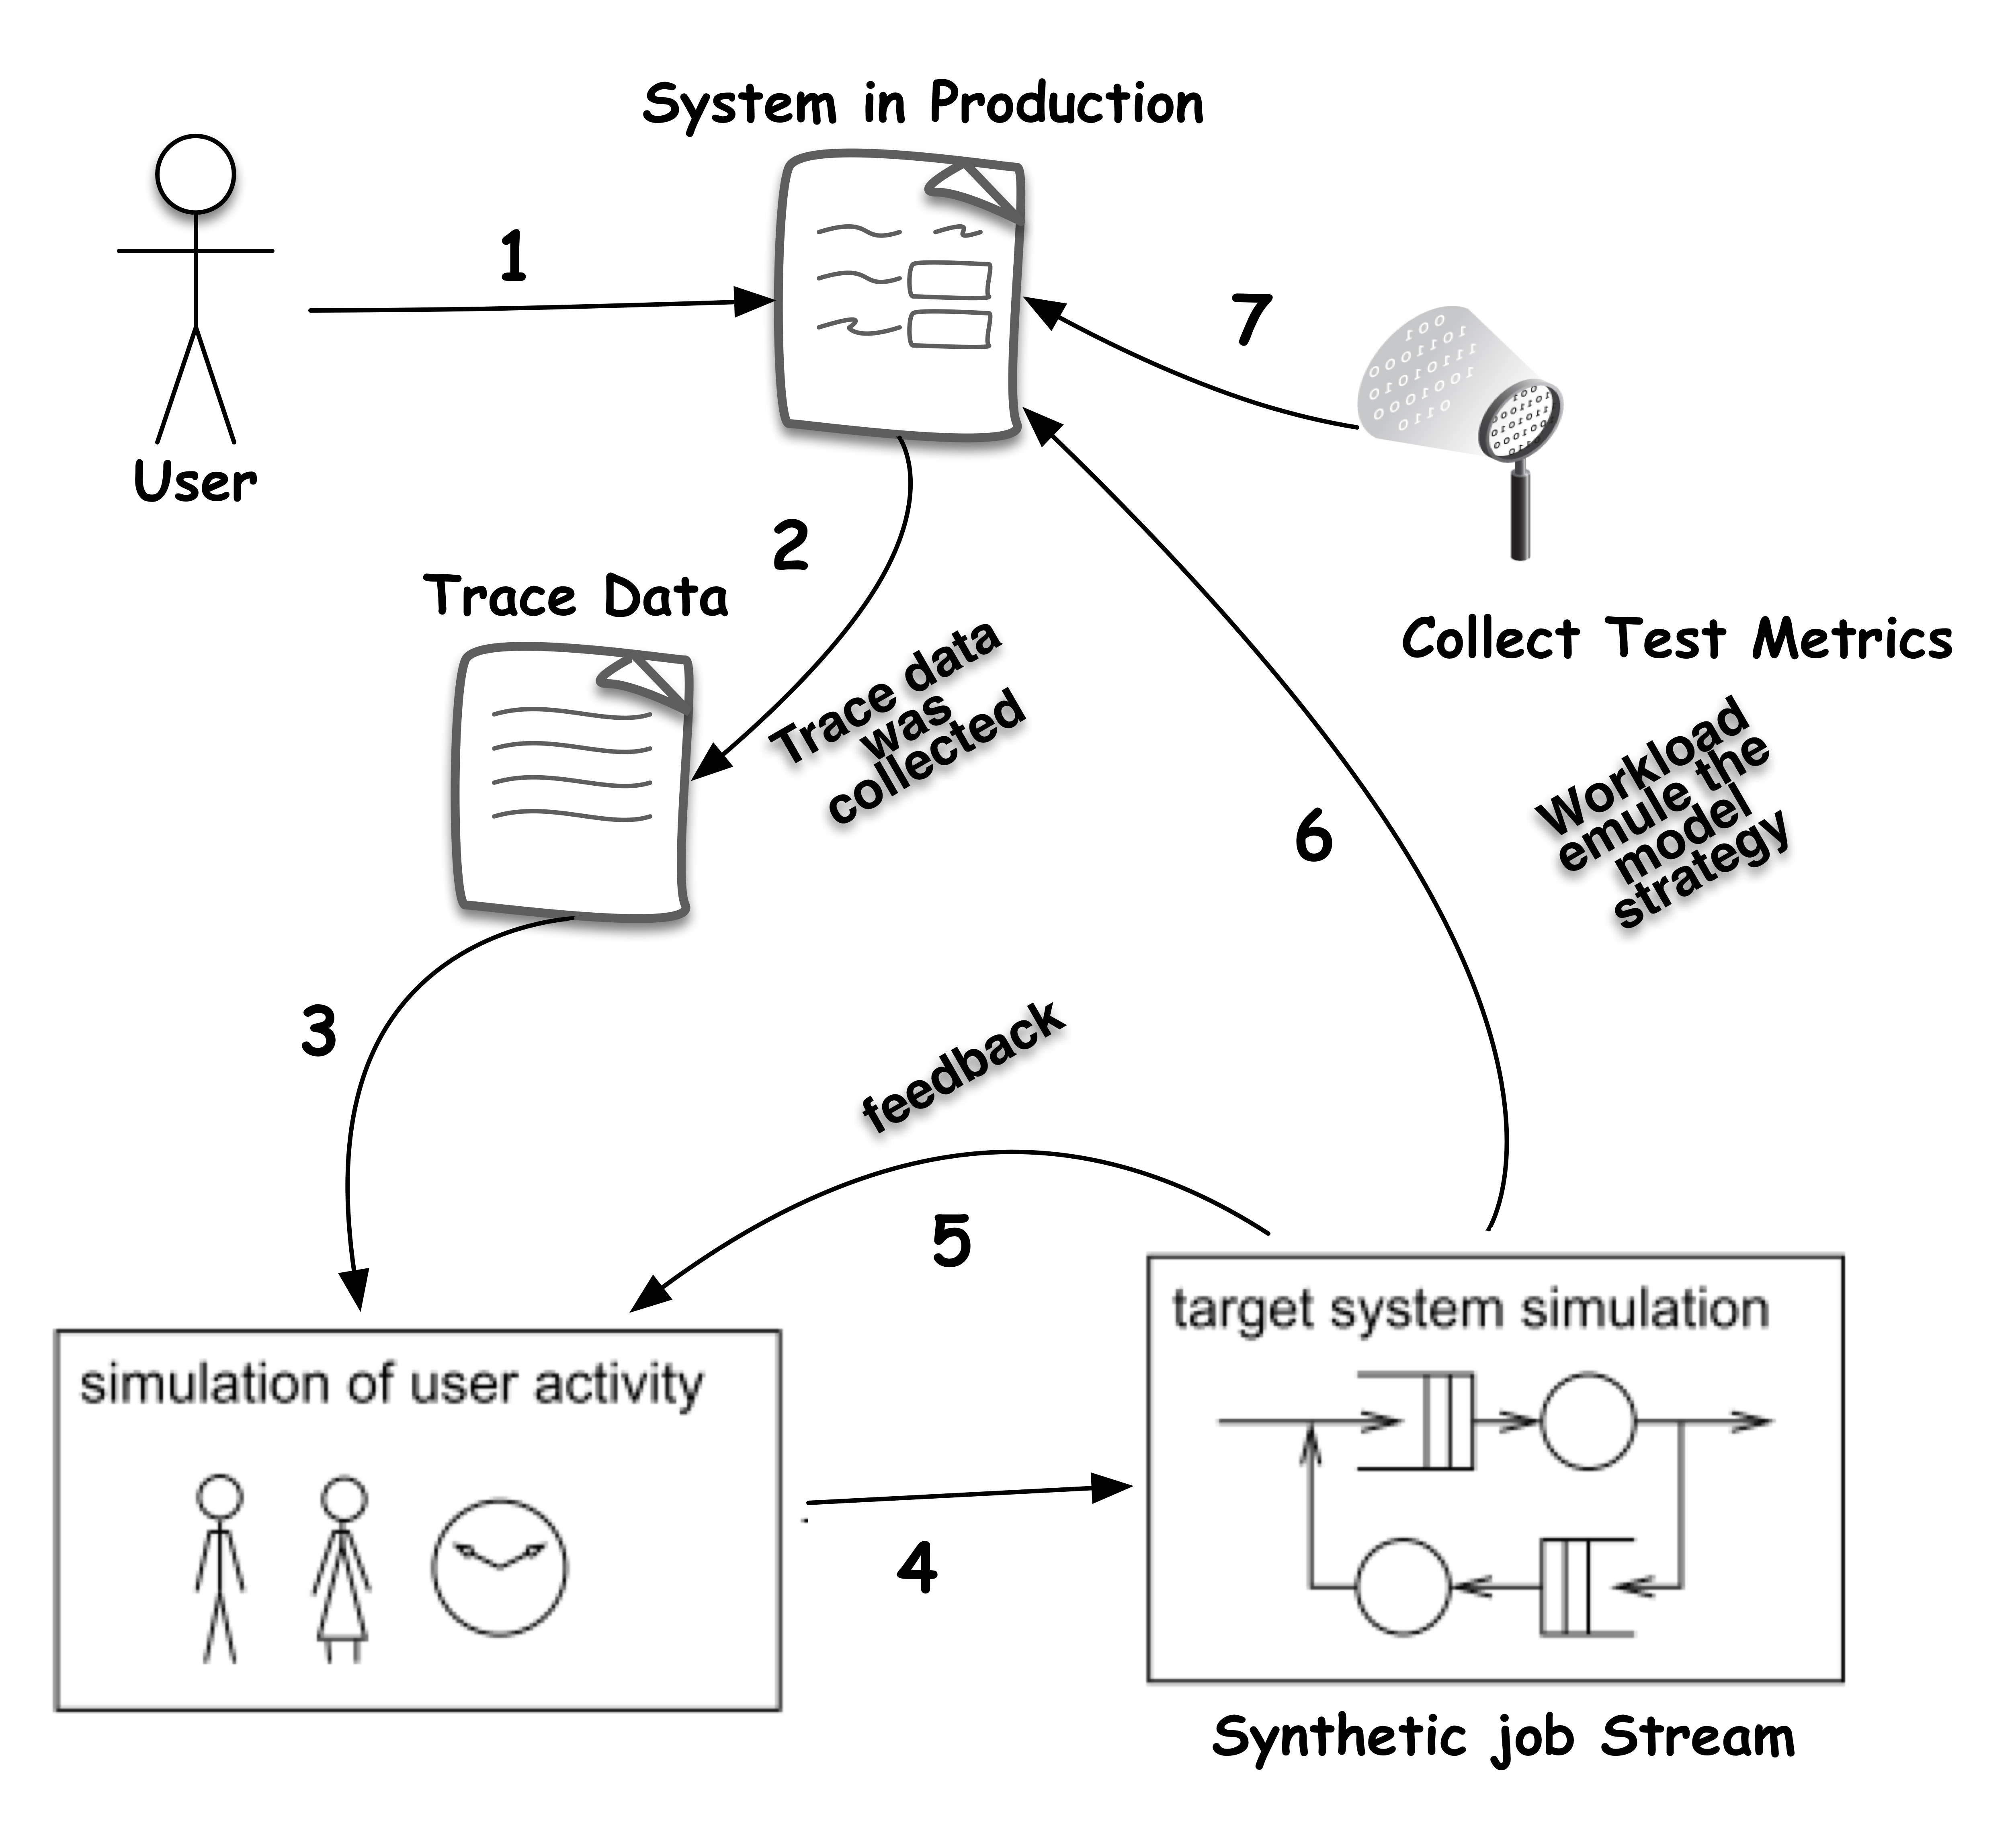
\includegraphics[width=0.8\textwidth]{./images/workloadmodel2300dpi.png}
\caption{Workload modeling based on the generative model \cite{DiLucca2006}}
\label{fig:generativemodel}

\end{figure}

Both load model have their advantages and disadvantages. In general, loads resulting from realistic-load based design techniques (Descriptive models) can be used to detect both functional and non-functional problems. However, the test durations are usually longer and the test analysis is more difficult. Loads resulting from fault-inducing load design techniques (Generative models) take less time to uncover potential functional and non-functional problems, the resulting loads usually only cover a small portion of the testing objectives \cite{Jiang2010}. The presented research work uses a generative model.


There are  several approaches to design generative or descriptive workloads:

\begin{itemize}
\item Model-based Stress testing: a usage model is proposed to simulate users’ behaviors.
\item Feedback-Directed Learning Software Testing: is an adaptive, feedback-directed learning testing system that learns rules from system execution \cite{Luo2015} \cite{Wert2014}.
\item Search-based Stress testing. 
\end{itemize}


Search-Based Stress testing will be detail explained in the chapter 3.

\subsection{Model-based Stress Testing}

Model-based testing is an application  of models to represent the desired behavior of a System Under Test or to represent testing strategies in a test. Some research aproaches proposes models to simulate or  generate realistic loads. Model-based testing (MBT) is a variant of testing that relies on explicit behaviour models that encode the intended behaviours of a system under test. Test cases are generated from one of these models or their combination \cite{MarkUtting2012} \cite{Bertolino2008}. 

The model paradgim is what paradigm and notation are used to describe the model. There are many different modelling notations that have been used for modelling the behaviour of systems for test generation purposes \cite{MarkUtting2012}. These paradigms are also used in the MBT state of the art survey provided by Dias-Neto et al. The overview article of Hierons et al.  discusses many of these paradigms in more detail \cite{Hierons2009} \cite{MarkUtting2012}. 

\begin{itemize}
\item State-Based (or Pre/Post) Notations. These model a system as a collection of variables, which represent a snapshot of the internal state of the system, plus some operations that modify those variables. Each operation is usually defined by a precondition and a postcondition, or the postcondition may be written as explicit code that updates the state \cite{MarkUtting2012}.
\end{itemize}

A User Community Modeling Language (UCML) is a set of symbols that can be used to create visual system usage models and depict associated parameters \cite{Wang2013}. The Fig. \ref{fig:ucml} shows a sample where all users realize a login into the application unde test. Once logged in, 40\% of the users navigates on the aplication, 30\%  of the users realizes downloads. 20\% of users realizes uploads and 10\% of users performs deletions.



\begin{figure}[!ht]
\centering
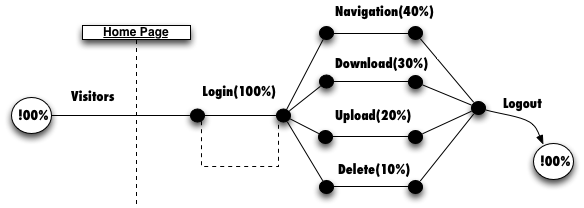
\includegraphics[width=1\textwidth]{./images/ucml.png}
\caption{User community modeling language \cite{Wang2013}}
\label{fig:ucml}

\end{figure}

Another technique to create workload models it is Stochastic Formcharts. The work of Draheim and Weber’s Formoriented analysis is a methodology for the specification of ultra-thin client based systems. Form-oriented models describe a web application as a bipartite state machine which consists of pages, actions, and transitions between them. Stochastic Formcharts are the combination of formoriented model and probability features. The Fig. \ref{fig:stform} shows a sample where all users have a probability of 100\% of realize a login into the application under test. Once logged in, users have a probability of 40\% of navigate on the application and so on \cite{Draheim2006b}.


\begin{figure}[!ht]
\centering
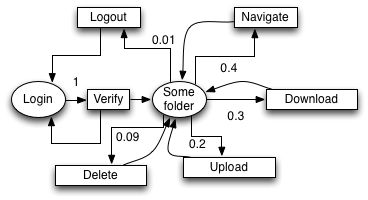
\includegraphics[width=0.8\textwidth]{./images/stochastic.png}
\caption{Stochastic Formcharts Example \cite{Draheim2006b} \cite{Wang2013}}
\label{fig:stform}
\end{figure}

One way to capture the navigational pattern within a session is through the Customer Behavior Model Graph (CBMG). Figure \ref{fig:cbmg} depicts an example of a CBMG showing that customers may be in several different states—Home, Browse, Search, Select, Add, and Pay—and they may transition between these states as indicated by the arcs connecting them. The numbers on the arcs represent transition probabilities. A state not explicitly represented in the figure is the Exit state \cite{Menasce2002a} \cite{Jiang2010} \cite{MohammadS.Obaidat}. 

\begin{figure}[!ht]
\centering
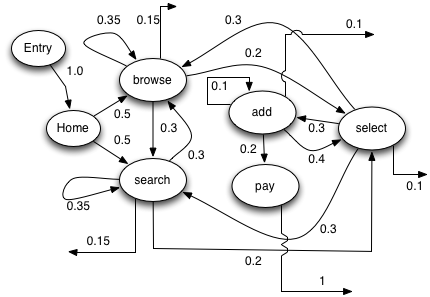
\includegraphics[width=0.8\textwidth]{./images/cbmg.png}
\caption{Example of a Customer Behavior Model Graph (CBMG)  \cite{Menasce2002a} \cite{Jiang2010} \cite{MohammadS.Obaidat}}
\label{fig:cbmg}
\end{figure}

Garousi et al. proposes derivate Stress Test Requirements from an UML model. The input model consists of a number of UML diagrams. Some of
them are standard in mainstream development methodologies and others are needed to describe the distributed architecture of the system under test (Fig. \ref{fig:modelbased}).

\begin{figure}[!ht]
\centering
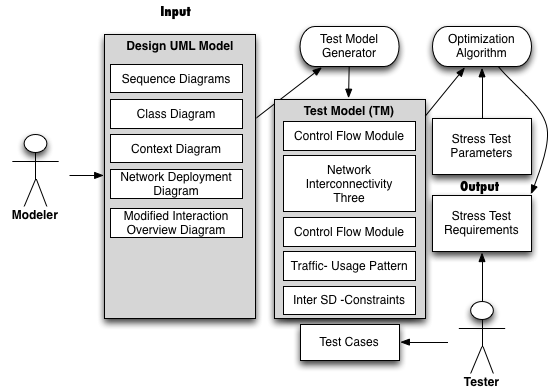
\includegraphics[width=1\textwidth]{./images/modelmethodology.png}
\caption{Model-based stress test methodology}
\label{fig:modelbased}
\end{figure}

Vogele et al. presents an approach that aims to automate the extraction and transformation of workload specifications for an model-based performance prediction of session-based application systems. The approach comprises three main components. First, a system- and tool-agnostic domain-specific language (DSL) allows the layered modeling of workload specifications of session-based systems. Second, instances of this DSL are automatically extracted. from recorded session logs of production systems. Third, these instances are transformed into executable workload specifications of load generation tools and model-based performance evaluation tools. We present transformations to the common load testing tool Apache JMeter and to the Palladio Component Model \cite{Vogele2016}.

\subsection{Feedback-Directed Learning Software Testing}

Feedback-ORiEnted PerfOrmance Software Testing (FOREPOST) is an adaptive, feedback-directed learning testing system that learns rules from system execution traces and uses these learned rules to select test input data automatically to find more performance problems in applications when compared to exploratory random performance testing \cite{Grechanik2012}.

FOREPOST uses runtime monitoring for a short duration of testing together with machine learning techniques and automated test scripts to reduce large amounts of performance-related information collected during AUT runs to a small number of descriptive rules that provide insights into properties of test input data that lead to increased computational loads of applications.

The Fig. \ref{fig:forepost} presents the main workflow of FOREPOST solution. The first step,  The Test Script is written  by the test engineer(1). Once the test script starts, its execution traces are collected (2) by the Profiler, and these traces are forwarded to the Execution Trace Analyzer, which produces (3) the Trace Statistics. The trace statistics is supplied (4) to Trace Clustering, which uses an ML algorithm, JRip to perform unsupervised clustering of these traces into two groups that correspond to (6) Good and (5) Bad test traces. 

The user can review the results of clustering (7). These clustered traces are supplied (8) to the Learner that uses them to learn the classification model and (9) output rules. The user can review (10) these rules and mark some of them as erroneous if the user has sufficient evidence to do so. Then the rules are supplied (11) to the Test Script. Finally, the input space is partitioned into clusters that lead to good and bad test cases, to find methods that are specific to good performance test cases. This task is accomplished in parallel to computing rules, and it starts when the Trace Analyzer produces (12) the method and data statistics that is used to construct (13) two matrices (14). Once these matrices are constructed, ICA decomposes them (15) into the matrices for bad and good test cases correspondingly. Finally, the Advisor (16) determines top methods that performance testers should look at (17) to debug possible performance problems.


\begin{figure}[!ht]
\centering
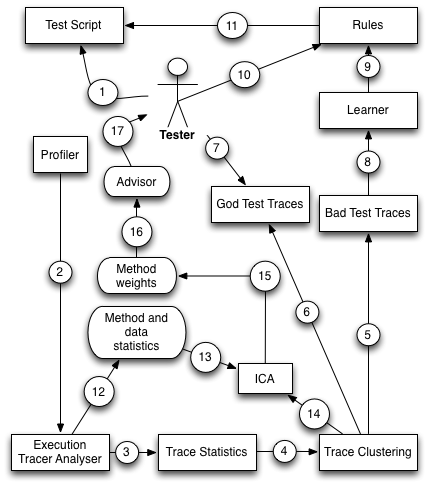
\includegraphics[width=0.7\textwidth]{./images/FOREPOST.png}
\caption{The architecture and workflow of FOREPOST}
\label{fig:forepost}
\end{figure}


\section{Research Question 2: How is a stress test executed and automated?}


The stress test execution  consists of deploy the system  and steup test execution ; generating the workloads according to the configurations and terminating the load when the load test is completed and recording the system behavior. There are three general approaches of load test executions \cite{Molyneaux2009}\cite{Jiang2010}:

\begin{itemize}
\item Live-User Based Executions: The test examines a system’s behavior when the system is simultaneously used by many users or execute a load test by employing a group of human testers. 
\item Driver Based Executions: The driver based execution approach automatically generate thousands or millions of concurrent requests for a long period of time using a software tool.
\item Emulation Based Executions: The emulation based load test execution approach performs the load testing on special platforms and doesn't require a fully functional system and conduct load testing.
\end{itemize}

Usually, a stress test execution it is performed with Driver Based Executions approach \cite{Erinle2013} \cite{MohammadS.Obaidat} \cite{Wang2013}. There are three categories of load drivers \cite{Jiang2010}: 

\begin{itemize}
\item Benchmark Suite: specialized load driver, designed for one type of system. For example, LoadGen is a load driver specified used to load test the Microsoft Exchange MailServer.
\item  Centralized Load Drivers: refer to a single load driver, which generates the load.
\item Peer-to-peer Load Drivers: refer to a set of load drivers, which collectively generate the target testing load. Peer-to-peer load drivers usually have a con- troller component, which coordinates the load generation among the peer load drivers. 
\end{itemize}


\subsection{Load Test Tools}

A stress test need to perform hundreds or thousands of concurrent requests  to the application under test. Automated tools are needed to carry out serious load, stress, and performance testing. Sometimes, there is simply no practical way to provide reliable, repeatable performance tests without using some form of automation. The aim of any automated test tool is to simplify the testing process. 

Workload generators are software products based on workload models to generate request sequences similar to real requests. They are designed and implemented as versatile software tools for performing tuning or capacity planning studies. Workload generators typically have the following components \cite{Molyneaux2009}:

\begin{itemize}
\item Scripting module: Enable recording of end-user activities in different middleware protocols;
\item Test management module: Allows the creation of test scenarios;
\item Load injectors: Generate the load with multiple workstations or servers;
\item Analysis module: Provides the ability to analyse the data collected by each test interation.
\end{itemize}


There are several tool to execution of Stress testing. In this tools, the procedure is semi-automated, whereas the execution of the tests itself is performed by a tool, the choice of scenarios to be executed as well as the decision to start new execution batteries are activities of the test designer or tester.

Normally, load test tools uses test scripts. Test scripts are written in a GUI testing framework or a backend server-directed performance tool such as JMeter. These frameworks are the basis on which performance testing is mostly done in industry. Performance test scripts imitate large numbers of users to create a significant load on the application under tests \cite{Grechanik2012}.

Comparing Web workload generators is a laborious and difficult task since they offer a large amount and diversity of features. In this section we contrast generators according to a wide set of features and capabilities, focusing on their ability to realize search-based tests or have learning capacities.

WebStone was designed by Silicon Graphics in 1996 to measure the perfor- mance of Web server software and hardware products. Nowadays, both executable and source actualized code for WebStone are available for free. The benchmark generates a Web server load by simulating multiple Web clients navigating a website. All the testing done by the benchmark is controlled by a Webmaster, which is a program that can be run on one of the client computers or on a different one \cite{MohammadS.Obaidat} \cite{Trent1995} . 

TPC Benchmarkt (TPC-W) is a transactional Web benchmark defined by the Transaction Processing Performance Council that models a representative e-commerce evaluating the architecture performance on a generic profile.The models uses a remote browser emulator to generate requests to server under test. TPC-W adopts the CBMG model to define the workloads in spite of this model only characterizing user dynamic behavior partially. The remote browser emulators are located in the client side and generate workload towards the e-commerce Web application, which is located in the server side (e-commerce server) \cite{MohammadS.Obaidat} \cite{Menasce2002a}.

\begin{figure}[h]
\centering
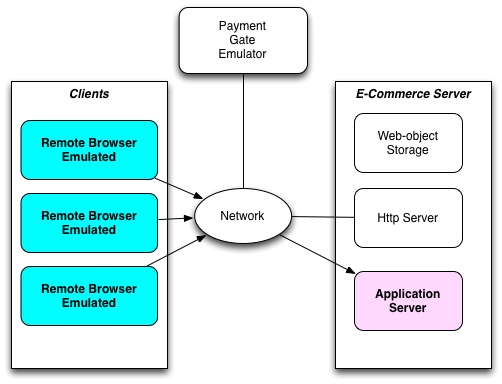
\includegraphics[width=0.8\textwidth]{./images/tpcw.png}
\caption{TPC-W architecture \cite{MohammadS.Obaidat} \cite{Menasce2002a}}
\label{fig:tpcw}
\end{figure}


Open STA is an open source software developed in C++, and released under the GPL licence. OpenSTA provides a script language which permits to simulate the activity of a user. This language can describe HTTP/S scenario and all the test executions is managed in a graphical interface. The composition of the test is
very simple, allowing the tester choose scripts for a test and a remote computer that will execute each test.


LoadRunner is one of the most popular industry-standard software products for functional and performance testing. It was originally developed by Mercury Interactive, but nowadays it is commercialized by Hewlett-Packard. LoadRunner supports the definition of user navigations, which are represented using a scripting language. The basic steps are recorded, creating a shell script. Next, this script is then taken off-line, and undergoes further manual steps such as data parameterization and correlations. Finally, the desired performance scripts are obtained after adding transactions and any other required logic (Fig. \ref{fig:loadrunner}). LoadRunner scripting only permits partial reproduction of user dynamism when generating Web workload, because it cannot define either advanced interactions of users, such as parallel browsing behavior, or continuous changes in user’s behaviors \cite{MohammadS.Obaidat}.

\begin{figure}[!ht]
\centering
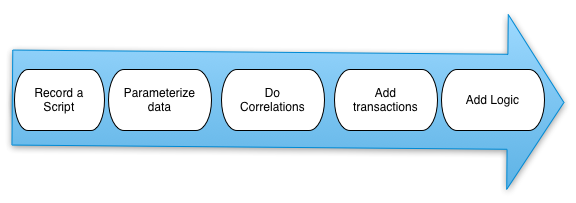
\includegraphics[width=1\textwidth]{./images/loadrunner.png}
\caption{Load Runner Scripting}
\label{fig:loadrunner}
\end{figure}



WebLOAD is a software tool for Web performance commercialized by RadView. It is oriented to explore the performance of critical Web applications by quantifying the utilization of the main server resources. The tool creates scenarios that try to mimic the navigations of real users. To this end, it provides facilities to record, edit and debug test scripts, which are used to define the scenarios on workload characterization. The execution environment is a console to manage test execution, whose results are analyzed in the Analytics application. Since WebLOAD is a distributed system, it is possible to deploy several load generators to reproduce the desired load. Load generators can also be used as probing clients where a single virtual user is simulated to evaluate specific statistics of a single user. These probing clients resemble the experience of a real user using the system while it is under load \cite{MohammadS.Obaidat}.

Apache JMeter is a free open source stress testing tool.  It has a large user base and offers lots of plugins to aid testing. JMeter is a desktop application designed to test and measure the performance and functional behavior of applications. The application it's purely Java-based and is highly extensible through a provided API (Application Programming Interface). JMeter works by acting as the client of a client/server application. JMeter allows multiple concurrent users to be simulated on the application \cite{Halili2008} \cite{Erinle2013}. 

JMeter has components organized  in a hierarchical manner. The Test Plan is the main component in a JMeter script. A typical test plan will consist of one or more Thread Groups, logic controllers, listeners, timers, assertions, and configuration elements:

\begin{itemize}
\item Thread Group: Test management module responsible to simulate the users used in a test. All elements of a test plan must be under a thread group.
\item Listeners: Analysis module responsible to provide access to the information gathered by JMeter about the test cases .
\item Samplers: Load injectors module responsible to send requests to a server, while Logical Controllers let you customize its logic.
\item Timers: allow JMeter to delay between each request.
\item Assertions: test if the application under test it is returning the correct results.
\item Configuration Elements: configure detais about the request protocol and test elements.
\end{itemize}


% Please add the following required packages to your document preamble:
% \usepackage[table,xcdraw]{xcolor}
% If you use beamer only pass "xcolor=table" option, i.e. \documentclass[xcolor=table]{beamer}
\begin{table}[h]
\centering
\caption{Comparison study presented by Pen˜a-Ortiz on the book Modeling and Simulation of Computer Networks and Systems Methodologies [F- Fully attended feature P-Partial attended feature] \cite{MohammadS.Obaidat} }
\label{tab:loadtool}
\begin{tabular}{llllll}
\rowcolor[HTML]{C0C0C0} 
\textbf{Feature}                                                                              & \textbf{Webstone}   & \textbf{SPECweb}                                                 & \textbf{SURGE}   & \textbf{Web polygraph} & \textbf{TPC-W}     \\
\begin{tabular}[c]{@{}l@{}}Analytical-Based\\ Architecture\end{tabular}                       & F                   & F                                                                & F                & F                      & F                  \\
\begin{tabular}[c]{@{}l@{}}Distributed\\ Architecture\end{tabular}                            & F                   & F                                                                & F                & F                      &                    \\
\begin{tabular}[c]{@{}l@{}}Business-Based\\ Architecture\end{tabular}                         &                     & P                                                                &                  & P                      & F                  \\
\begin{tabular}[c]{@{}l@{}}Client\\ Parameterization\end{tabular}                             & F                   & F                                                                &                  & P                      & F                  \\
Workload Types                                                                                &                     & F                                                                &                  &                        & F                  \\
Multi-platform                                                                                & F                   & F                                                                & F                & F                      & F                  \\
Open Source                                                                                   & F                   &                                                                  & F                & P                      & F                  \\
\rowcolor[HTML]{FFFC9E} 
\textbf{\begin{tabular}[c]{@{}l@{}}Search-based Testing\\  or Learning features\end{tabular}} & \textbf{}           & \textbf{}                                                        & \textbf{}        & \textbf{}              & \textbf{}          \\
\rowcolor[HTML]{C0C0C0} 
\textbf{Feature}                                                                              & \textbf{LoadRunner} & \textbf{WebLoad}                                                 & \textbf{JMeter}  & \textbf{S-Clients}     & \textbf{WebJammma} \\
\begin{tabular}[c]{@{}l@{}}Analytical-Based\\ Architecture\end{tabular}                       & P                   & P                                                                & P                &                        &                    \\
\begin{tabular}[c]{@{}l@{}}Distributed\\ Architecture\end{tabular}                            & F                   & F                                                                &                  &                        &                    \\
\begin{tabular}[c]{@{}l@{}}Business-Based\\ Architecture\end{tabular}                         & F                   & F                                                                & F                &                        &                    \\
\begin{tabular}[c]{@{}l@{}}Client\\ Parameterization\end{tabular}                             & F                   & F                                                                & F                &                        & F                  \\
Workload Types                                                                                & F                   & F                                                                & P                &                        &                    \\
Multi-platform                                                                                & F                   & F                                                                & F                & F                      & F                  \\
Open Source                                                                                   &                     &                                                                  & F                & F                      & F                  \\
\rowcolor[HTML]{FFFC9E} 
\textbf{\begin{tabular}[c]{@{}l@{}}Search-based Testing\\  or Learning features\end{tabular}} & \textbf{}           & \textbf{}                                                        & \textbf{}        & \textbf{}              & \textbf{}          \\
\rowcolor[HTML]{C0C0C0} 
\textbf{Feature}                                                                              & \textbf{Deluge}     & \textbf{\begin{tabular}[c]{@{}l@{}}HAMMER\\ HEAD 2\end{tabular}} & \textbf{PTester} & \textbf{Siege}         & \textbf{Locust}    \\
\begin{tabular}[c]{@{}l@{}}Analytical-Based\\  Architecture\end{tabular}                      &                     &                                                                  &                  &                        & P                  \\
\begin{tabular}[c]{@{}l@{}}Distributed\\ Architecture\end{tabular}                            &                     &                                                                  &                  &                        &                    \\
\begin{tabular}[c]{@{}l@{}}Business-Based\\ Architecture\end{tabular}                         &                     &                                                                  &                  &                        & F                  \\
\begin{tabular}[c]{@{}l@{}}Client\\ Parameterization\end{tabular}                             &                     &                                                                  &                  &                        & F                  \\
Workload Types                                                                                &                     &                                                                  &                  &                        & P                  \\
Multi-platform                                                                                & F                   & P                                                                & F                & P                      & F                  \\
Open Source                                                                                   & F                   & F                                                                & F                & F                      & F                  \\
\rowcolor[HTML]{FFFC9E} 
\textbf{\begin{tabular}[c]{@{}l@{}}Search-based Testing\\  or Learning features\end{tabular}} & \textbf{}           & \textbf{}                                                        & \textbf{}        & \textbf{}              & \textbf{}         
\end{tabular}
\end{table}

Table \ref{tab:loadtool} summarizes the studied workloads generators as well as the grade (full or partial) in which they fulfill the features described bellow.

\section{Research Question 3: What are the main problems found by stress tests?}

 Performance problems share common symptoms and many performance problems described in the literature are defined by a particular set of root causes. Fig. \ref{fig:symptoms}  shows the symptoms of known performance problems \cite{Wert2013a}. 



\begin{figure}[h]
\centering
\includegraphics[width=0.8\textwidth]{./images/symptoms.png}
\caption{Symptoms of know performance problems \cite{Wert2013a}. }
\label{fig:symptoms}
\end{figure}


There are several antipatterns that details features about  common performance problems. Antipatterns are conceptually similar to patterns in that they document recurring solutions to common design problems. They are known as
antipatterns because their use produces negative consequences.  Performance antipatterns document common performance mistakes made in software architectures or designs. These software Performance antipatterns have four primary uses: identifying problems,
focusing on the
right level of abstraction,
effectively communicating
their causes to others, and prescribing solutions \cite{brown1998antipatterns}. The table \ref{antipatterns} present some of the most common performance antipatterns.


% Please add the following required packages to your document preamble:
% \usepackage{multirow}
% \usepackage[table,xcdraw]{xcolor}
% If you use beamer only pass "xcolor=table" option, i.e. \documentclass[xcolor=table]{beamer}
\begin{table}[H]
\centering
\caption{Performance antipatterns}
\label{antipatterns}
\begin{tabular}{|l|l|}
\hline
\rowcolor[HTML]{C0C0C0} 
\multicolumn{1}{|c|}{\cellcolor[HTML]{C0C0C0}\textbf{antipattern}} & \multicolumn{1}{c|}{\cellcolor[HTML]{C0C0C0}\textbf{Derivations}} \\ \hline
Blob or The God Class &  \\ \hline
 & Concurrent processing Systems \\ \cline{2-2} 
 & Piper and Filter Architectures \\ \cline{2-2} 
\multirow{-3}{*}{Unbalanced-Processing} & Extensive Processing \\ \hline
Circuitous Treasure Hunt &  \\ \cline{1-1}
Empty Semi Trucks &  \\ \cline{1-1}
Tower of Babel &  \\ \cline{1-1}
One-Lane Bridge &  \\ \cline{1-1}
Excessive Dynamic Allocation &  \\ \cline{1-1}
Traffic Jam &  \\ \cline{1-1}
The Ramp  &  \\ \cline{1-1}
More is Less & \multirow{-10}{*}{} \\ \hline
\end{tabular}
\end{table}

Blob antipattern is known by various names, including the “god” class [8] and the “blob” [2]. Blob is an antipattern whose problem is on the excessive message traffic generated by a single class or component, a particular resource does the majority of the work in a software. The Blob antipattern occurs when a single class or component either performs all of the work of an application or holds all of the application’s data. Either manifestation results in excessive message traffic that can degrade performance \cite{Cortellessa2007} \cite{Smith2000}.

A project containing a “god” class is usually has a single, complex controller class that is surrounded by simple classes that serve only as data containers. These classes typically contain only accessor operations (operations to get() and set() the data) and perform little or no computation of their own \cite{Smith2000}.
The  Figures \ref{fig:godclass} and \ref{fig:godclass2} describes an hypotetical system with a BLOB problem:
The Fig. \ref{fig:godclass} presents a sample where the Blob class uses the features A,B,C,D,E,F and G of the hypotetical system; The Fig. \ref{fig:godclass2}  shows a static view where  a complex software entity instance, i.e. Sd, is connected to other software instances, e.g. Sa, Sb and Sc, through many dependencies \cite{Vetoio2011}\cite{Wert2013a}.




\begin{figure}[h]
\centering
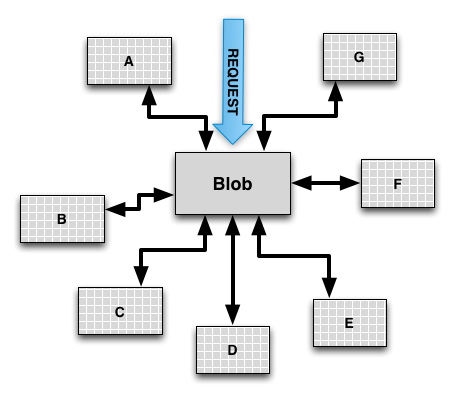
\includegraphics[width=0.8\textwidth]{./images/BLOB.png}
\caption{The God class\cite{Wert2013a}. }
\label{fig:godclass}
\end{figure}
\begin{figure}[h]
\centering
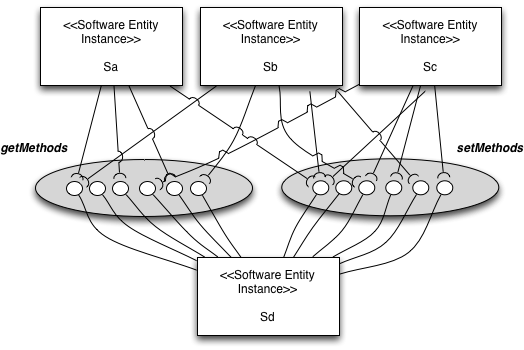
\includegraphics[width=0.8\textwidth]{./images/blob2.png}
\caption{The God class\cite{Vetoio2011}. }
\label{fig:godclass2}
\end{figure}

Unbalanced Processing it's characterises for one scenario where a specific class of requests generates a pattern of execution within the system that tends to overload a particular resource. In other words the overloaded resource will be executing a certain type of job very often, thus in practice damaging other classes
of jobs that will experience very long waiting times. Unbalanced Processing occurs in three different situations. The first case that cause unbalanced processing it is when processes cannot make effective use of available processors either because processors are dedicated to other tasks or because of single-threaded code. This manifestation has available processors and we need to ensure that the software is able to use them. Fig. \ref{fig:unbalanced}  shows a sample of the Unbalanced Processing. In The Fig. \ref{fig:unbalanced}, four tasks are performed. The task D it is waiting for the task C conclusion that are submmited to a heavy processing situation. 

The pipe and filter architectures  and extensive processing antipattern represents a manifestation of the unbalanced processing antipattern. The pipe and filter architectures occurs when the throughput of the overall system is determined by the slowest filter. The  Fig. \ref{fig:pipefilter} describes a software S with a Pipe and Filter Architectures problem: (a) Static View, there is a software entity instance, e.g. Sa, offering an operation (operation x) whose resource demand (computation = \$compOpx, storage = \$storOpx, bandwidth = \$bandOpx) is quite high; (b) Dynamic View, the operation opx is invoked in a service  and the throughput of the service (\$Th(S)) is lower than the required one. The extensive processing occurs when a process monopolizes a processor and prevents a set of other jobs to be executed until it finishes its computation. The Fig. \ref{fig:extpro} describes a software S with a Extensive Processing problem: (a) Static View, there is a software entity instance, e.g. Sa, offering two operations (operation x, operation y) whose resource demand is quite unbalanced, since opx has a high demand (computation = \$compOpx, storage = \$storOpx, bandwidth = \$bandOpx), whereas opy has a low demand (computation = \$compOpy, storage = \$storOpy, bandwidth = \$bandOpy); (b) Dynamic View, the operations opx and opy are alternatively invoked in a service and the response time of the service (\$RT(S)) is larger than the required one \cite{Vetoio2011}.

\begin{figure}[h]
\centering
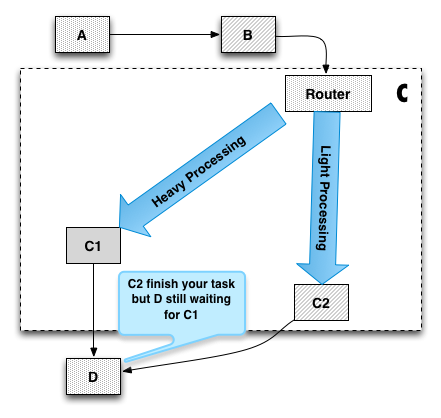
\includegraphics[width=0.5\textwidth]{./images/unbalanced.png}
\caption{Unbalanced Processing sample \cite{Wert2013a}. }
\label{fig:unbalanced}
\end{figure}


\begin{figure}[h]
\begin{minipage}{.5\textwidth}
\centering
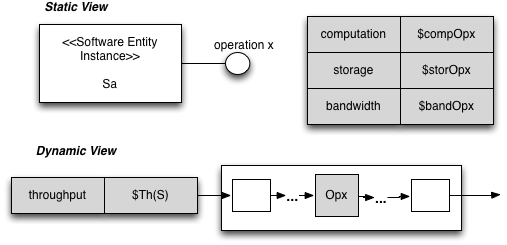
\includegraphics[width=1\textwidth]{./images/pipe2.png}
\caption{Pipe and Filter sample \cite{Vetoio2011}}
\label{fig:pipefilter}
\end{minipage}
\begin{minipage}{.5\textwidth}
\centering
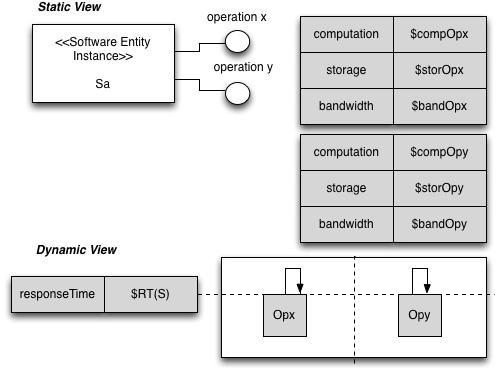
\includegraphics[width=1\textwidth]{./images/extpro.png}
\caption{Extensive Processing sample \cite{Vetoio2011}.}
\label{fig:extpro}
\end{minipage}
\end{figure}


Circuitous Treasure Hunt antipattern occurs when software retrieves data from a first componet, uses those results in a second component, retrieves data from the second component, and so on, until the last results are obtained \cite{Smith2002} \cite{Smith2003}. Circuitous Treasure Hunt 
are typical performance antipatterns that causes unnecessarily frequent database requests. The Circuitous Treasure Hunt antipattern is a result from a bad database schema or query design. A common Circuitous Treasure Hunt design creates a data dependency between single queries. For instance, a query requires the
result of a previous query as input. The longer the chain of
dependencies between individual queries the more the Circuitous
Treasure Hunt antipattern hurts performance \cite{Wert2014}. The Fig. \ref{fig:circuit}  shows a software S with a Circuitous Treasure Hunt problem: (a) Static View, there is a software entity instance e.g. Sa, retrieving information from the database; (b) Dynamic View, the software  S generates a large number of database calls by performing several queries up to the final operation \cite{Vetoio2011}.


\begin{figure}[h]
\centering
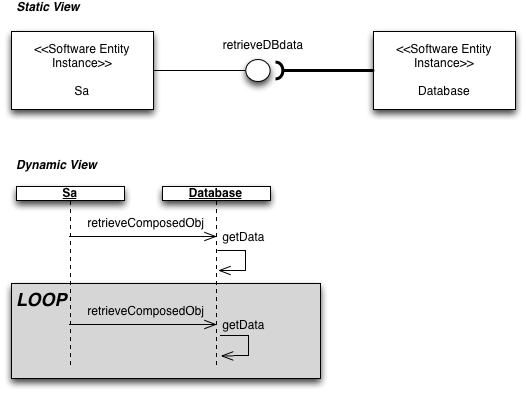
\includegraphics[width=1\textwidth]{./images/circuit.png}
\caption{Circuitous
Treasure Hunt sample \cite{Vetoio2011}}
\label{fig:circuit}
\end{figure}


\begin{figure}[h]
\centering
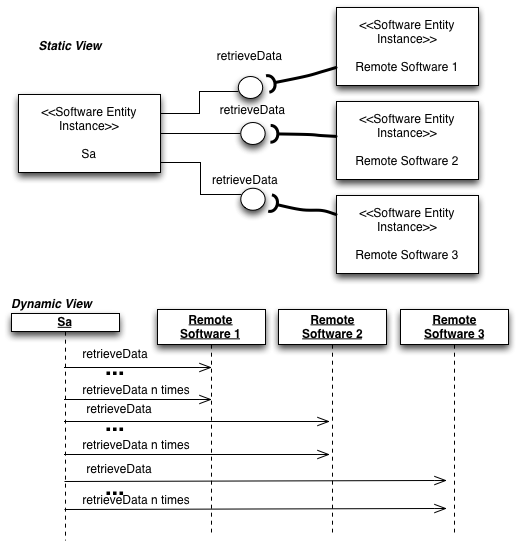
\includegraphics[width=0.8\textwidth]{./images/trucks.png}
\caption{Empty Semi Trucks sample \cite{Vetoio2011}.}
\label{fig:trucks}
\end{figure}

Empty Semi Trucks occurs when an excessive number of requests is required to perform a task. It may be due to inefficient use of available bandwidth, an inefficient interface, or both \cite{Arcelli2012}. There are a special case of Empty Semi Trucks that occurs  when many fields in a user interface must be retrieved from a
remote system. Fig. shows a software S with a Empty Semi Trucks problem: (a) Static View, there is a software entity instance, e.g. Sa, retrieving some information from several instances (Remote Software 1, . . . , Remote Software n); (b) Dynamic View, the software instance Sa generates an excessive message traffic by sending a big amount of messages with low sizes, much lower than the network bandwidth, hence the network link might have a low utilization value \cite{Vetoio2011}.

The Tower of Babel antipattern most often occurs when information is translated into an exchange format, such as XML, by the sending process then parsed and translated into an
internal format by the receiving process. When the translation and parsing is excessive, the system spends most
of its time doing this and relatively little doing real work \cite{Smith2003}. Fig. shows a system with a Tower of Babel problem: (a) Static View, there are some software entity instances, e.g. Sa, Sb, . . . , Sn; (b) Dynamic View, the software instances Sd performs many times the translation of format for communicating with other instances \cite{Vetoio2011}.

\begin{figure}[h]
\centering
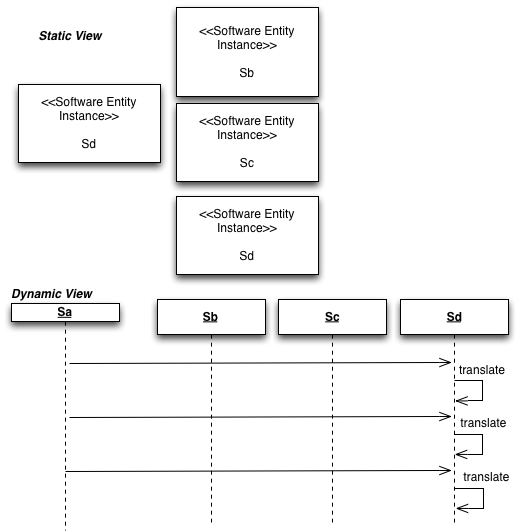
\includegraphics[width=0.6\textwidth]{./images/babel2.png}
\caption{Tower of Babel sample \cite{Vetoio2011}}
\label{fig:babel}
\end{figure}

\begin{figure}[h]
\centering
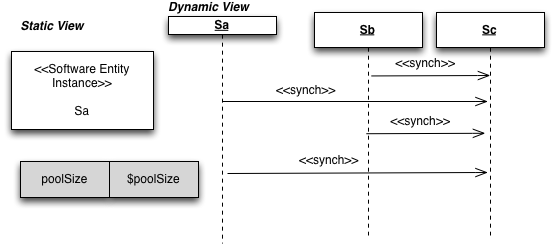
\includegraphics[width=1\textwidth]{./images/onelane.png}
\caption{One-Lane Bridge sample \cite{Vetoio2011}.}
\label{fig:onelane}

\end{figure}


One-Lane Bridge is a antipattern that occurs when one or a few processes execute concurrently using a shared resource and other processes are waiting for use the shared resource. It frequently occurs in applications that access a database. Here, a lock ensures that only one process may update the associated portion of the database at a time. This antipatterns is common when many concurrent threads or processes are waiting for the same shared resources. These can either be passive resources (like semaphores or mutexes) or active resources (like CPU or hard disk). In the first case, we have a typical One Lane Bridge whose critical resource needs to be identified. Figure 3.10 shows a system with a One-Lane Bridge problem: (a) Static View, there is a software entity instance with a capacity of managing \$poolSize threads; (b) Dynamic View, the software instance Sc receives an excessive number of synchronous calls in a service S and the predicted response time is higher than the required \cite{Vetoio2011}.


Using dynamic allocation, objects are created when they are first accessed and then destroyed when they are no longer needed. Excessive Dynamic Allocation, however, addresses frequent, unnecessary creation and destruction of objects of the same class. Dynamic allocation is expensive , an object created in memory must be allocated from the heap, and any initialization code for the object and the contained objects must be executed. When the object is no longer needed, necessary clean-up must be performed, and the reclaimed memory must be returned to the heap to avoid memory leaks \cite{Smith2002} \cite{Smith2003}.

\begin{figure}[H]
\begin{minipage}{.5\textwidth}
\centering
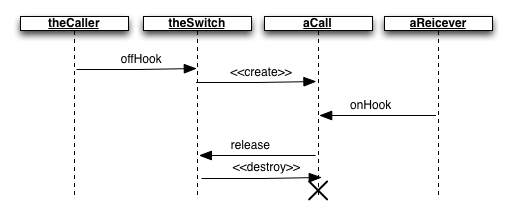
\includegraphics[width=1\textwidth]{./images/excessivedynamicallocation.png}
\caption{Excessive Dynamic Allocation.}
\label{fig:dynallocation}
\end{minipage}
\begin{minipage}{.5\textwidth}
\centering
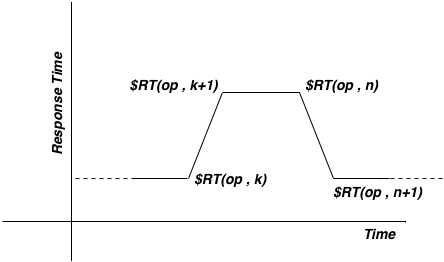
\includegraphics[width=1\textwidth]{./images/jam.png}
\caption{Traffic Jam Response Time \cite{Vetoio2011}.}
\label{fig:jam}
\end{minipage}
\end{figure}

The Fig. \ref{fig:dynallocation} shows a Excessive Dynamic Allocation sample. This example is drawn from a call (an offHook event), the switch creates a Call object to manage the call. When the call is completed, the Call object is destroyed. Constructing a single Call object it is not seem as excessive. A Call is a complex object that contains several other objects that must also be created. The Excessive Dynamic Allocation occurs when  a switch receive hundreds of thousands of offHook events. In a case like this, the overhead for dynamically allocating call objects adds substantial delays to the time needed to complete a call.

The Traffic Jam antipattern occurs if many concurrent threads or processes are waiting for the same  active resources (like CPU or hard disk). This antipatterns produces a large backlog in jobs waiting for service. The performance impact of the Traffic Jam is the transient behavior that produces wide variability in response time. Sometimes it is fine, but at other times, it is unacceptably long. Figure \ref{fig:jam} describes a software with a Traffic Jam problem, the monitored response time of the operation shows a wide variability in response time which persists long \cite{Vetoio2011}. 


\begin{figure}[H]
\begin{minipage}{.5\textwidth}
\centering
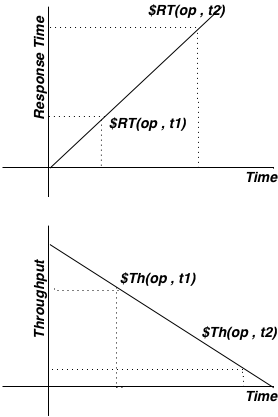
\includegraphics[width=0.5\textwidth]{./images/ramp.png}
\caption{The Ramp sample \cite{Vetoio2011}.}
\label{fig:ramp}
\end{minipage}
\begin{minipage}{.5\textwidth}
\centering
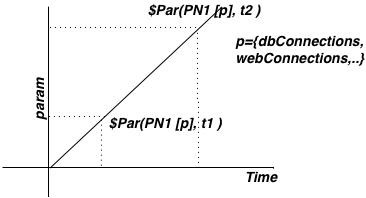
\includegraphics[width=1\textwidth]{./images/moreisless.png}
\caption{More is Less sample \cite{Vetoio2011}.}
\label{fig:moreisless}
\end{minipage}
\end{figure}

The Ramp it is a antipattern where the processing time increases as the system is used. The Ramp can arise in several different ways. Any situation in which the amount of processing required to satisfy a request increases over time will produce the behavior. With the Ramp antipattern, the memory consumption of the application is growing over time. The root cause is Specific Data Structures which are growing during operation or which are not properly disposed \cite{Wert2014} \cite{Smith2003}. Fig. \ref{fig:ramp} shows a system  with The Ramp problem:  (i) the monitored response time of the operation opx at time t1, i.e. \$RT(opx, t1), is much lower than the monitored response time of the operation opx at time t2, i.e. \$RT(opx, t2), with t1 < t2; (ii) the monitored throughput of the operation opx at time t1, i.e. \$Th(opx, t1), is much larger than the monitored throughput of the operation opx at time t2, i.e. \$Th(opx, t2), with t1 < t2. 

More is less occurs when a system spends more time "thrashing” than accomplishing real work because there are too many processes relative to available resources. More is Less are presented when it is running too many programs overtime. This antipattern causes too much system paging and systems spend all their time servicing page faults rather than processing requests. In distributed systems, there are more causes.They include: creating too many database connections and  allowing too many internet connection. Fig. \ref{fig:moreisless} describes a system  with a More Is Less problem: There is a processing node PN1 and the monitored runtime parameters (e.g. database connections, etc.) at time t1, i.e. \$Par(PN1[p], t1), are much larger than the same parameters at time t2, i.e. \$Par(PN1[p], t2), with t1 < t2. 


\section{Research Question 4: How are the stress tests results analysed?}

The system behavior recorded during the stress test execution phase needs to be analyzed to determine if there are any load-related functional or non-functional problems \cite{Jiang2010}. 


There can be many formats of system behavior like resource usage data or end-to-end response time, which is recorded as response time for each individual request. These types of data need to be processed before comparing against threshold values. A proper data summarization technique is needed to describe these many data instances into one number. 


There are three types of data summarization techniques proposed in the literature. Jiang et al. use response time analysis as an example to describe the proposed data summarization techniques \cite{Jiang2010}:

\begin{itemize}
\item Maximum values;
\item Average or Medium Vales;
\item Percentile-values. 
\end{itemize}


Some researchers advocate that the 90-percentile response time is a better measurement than the average/medium response time, as the former accounts for most of the peaks, while eliminating the outliers \cite{Jiang2010}.


\section{Conclusion}


% Please add the following required packages to your document preamble:
% \usepackage[table,xcdraw]{xcolor}
% If you use beamer only pass "xcolor=table" option, i.e. \documentclass[xcolor=table]{beamer}
\begin{table}[H]
\centering
\caption{My caption}
\label{my-label}
\begin{tabular}{lllllll}
\rowcolor[HTML]{C0C0C0} 
\textbf{Test Design}                                                                   & \textbf{\begin{tabular}[c]{@{}l@{}}Test \\ Execution\end{tabular}}                 & \textbf{Load Driver}                                                                       & \textbf{\begin{tabular}[c]{@{}l@{}}Test Tool \\ License\end{tabular}} & \textbf{\begin{tabular}[c]{@{}l@{}}Search-Based \\ Stress Test \\ Application\end{tabular}} & \textbf{\begin{tabular}[c]{@{}l@{}}Search-Based \\ Test \\ Metaheuris.\end{tabular}}         & \textbf{\begin{tabular}[c]{@{}l@{}}Test \\ Results\end{tabular}}                  \\
\begin{tabular}[c]{@{}l@{}}Model-Based\\ Testing\end{tabular}                          & \begin{tabular}[c]{@{}l@{}}Live-User\\ Based\end{tabular}                          & \begin{tabular}[c]{@{}l@{}}Benchmark\\ Suite\end{tabular}                                  & Comercial                                                             & Real-Time                                                                                   & \cellcolor[HTML]{9AFF99}\begin{tabular}[c]{@{}l@{}}Genetic \\ Algorithms\\ (GA)\end{tabular} & Average                                                                           \\
FOREPOST                                                                               & \cellcolor[HTML]{9AFF99}\begin{tabular}[c]{@{}l@{}}Driver-\\ Based\end{tabular}    & \begin{tabular}[c]{@{}l@{}}Centralized \\ L. Drivers\end{tabular}                          & \cellcolor[HTML]{9AFF99}Open-source                                   & \cellcolor[HTML]{9AFF99}Industrial                                                          & \cellcolor[HTML]{9AFF99}\begin{tabular}[c]{@{}l@{}}Simulated\\ Annealing\end{tabular}        & \cellcolor[HTML]{9AFF99}\begin{tabular}[c]{@{}l@{}}90- \\ Percentile\end{tabular} \\
\cellcolor[HTML]{9AFF99}\begin{tabular}[c]{@{}l@{}}Search-Based\\ Testing\end{tabular} & \cellcolor[HTML]{9AFF99}\begin{tabular}[c]{@{}l@{}}Emulation-\\ Based\end{tabular} & \cellcolor[HTML]{9AFF99}\begin{tabular}[c]{@{}l@{}}Peer-to-peer \\ L. Drivers\end{tabular} &                                                                       &                                                                                             & \cellcolor[HTML]{9AFF99}Tabu Search                                                          & \cellcolor[HTML]{9AFF99}\begin{tabular}[c]{@{}l@{}}80-\\ Percentile\end{tabular}  \\
                                                                                       &                                                                                    &                                                                                            &                                                                       &                                                                                             & Ant Colony                                                                                   & \cellcolor[HTML]{9AFF99}\begin{tabular}[c]{@{}l@{}}70- \\ Percentile\end{tabular} \\
                                                                                       &                                                                                    &                                                                                            &                                                                       &                                                                                             & \begin{tabular}[c]{@{}l@{}}Particle \\ Swarm\end{tabular}                                    & \cellcolor[HTML]{9AFF99}Maximum                                                   \\
                                                                                       &                                                                                    &                                                                                            &                                                                       &                                                                                             & \begin{tabular}[c]{@{}l@{}}Hill \\ Climbing\end{tabular}                                     & \cellcolor[HTML]{9AFF99}Minimal                                                  
\end{tabular}
\end{table}

